% !TEX root = ../main.tex
\section{Beyond First Level} \label{ssec::beyondfirstlevel}
\DndDropCapLine{W}{ith one heavy loss, the group}
dispatches the fearsome troll.
They perform a small funerary ritual, to then finally get some rest.
Beaten and tired, they learned their lesson for the day.

% TODO: Add more flavor text or add stuff here and there to fill the page.

\thispagestyle{empty}
\begin{tikzpicture}[remember picture,overlay]
    \node[anchor=south, yshift=-0.10cm] at (current page.south) {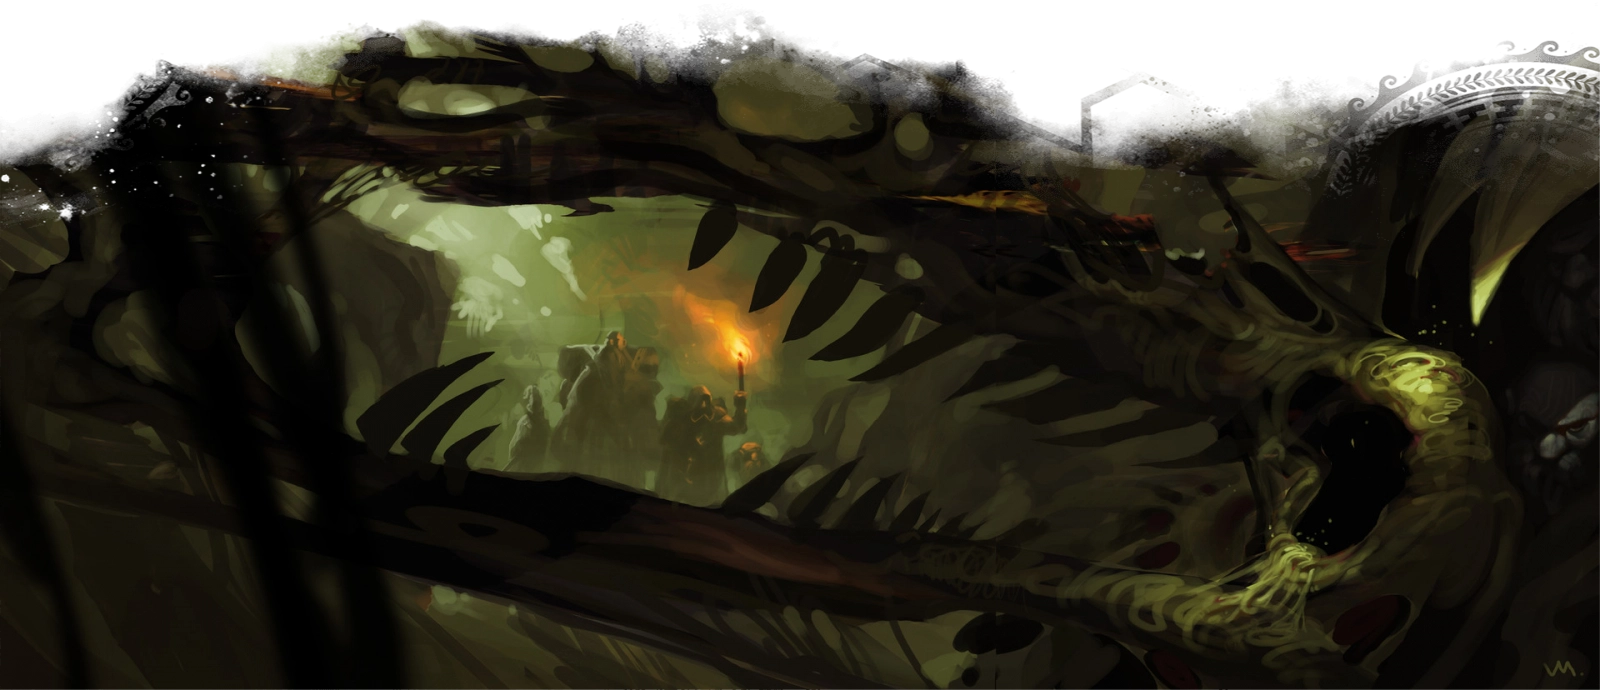
\includegraphics[width=\pdfpagewidth]{06classless/img/10jungle_adventure}};
\end{tikzpicture}

\subsubsection{Experience}
    What is learned by your character during the game is measured by Experience Points (XP).
    After you finish playing, talk about the session with the whole group and discuss what happened.
    Read the questions in the table below.
    For each of them that you can reply ``yes'' to, your character gets one XP.

    \begin{itemize}
        \item Did you participate in the session?
        \item Did you travel to a new location?
        \item Did you defeat one or more creatures?
        \item Did you loot treasure?
        \item Did you complete a quest?
        \item Did you solve a conflict?
        \item Did you make a new friend, ally, or enemy?
        \item Did you help another PC?
        \item Did your ideals, bonds, or flaws affect any of your decisions during the session?
        \item Did you perform any action related to your kin, background, or origin?
        \item Did you perform an extraordinary action of some kind?
    \end{itemize}

    In case of any discussion or disagreement, the DM always has the last word.
    Additional XP may be awarded when specific story milestones are achieved, but this too is left to the discression of the DM.

    \newpage

\subsubsection{Feat Points}
    As your character adventures, they will gain \textbf{Feat Points} (FP).
    Feat points are spent to buy feats, which can only be done as part of a long rest.
    You can buy multiple feats in one long rest.
    Feats either increase your proficiency level at a skill or a proficiency, or they include a useful feature.

    When you reach 10 XP, reset your XP counter and add one FP, keeping the remaining XP.
    Feat points are used to learn new feats, which include either an increase in a proficiency level or a feature.

    You don't need to spend FP right after earning it, you can save as many as you want for as long as you need.
    The full list of feats starts in the next page.

\subsubsection{Leveling Up}
    As your character gains feat points they will gain levels, acquiring hit dice, improving their ability scores and saving throw proficiencies, and gaining major character advancements.
    \begin{itemize}
        \item Ability Score Improvements allow you to increase one of you ability scores by 1.
        \item Saving Throw Improvements increase your level of proficiency on a saving throw of your choice by 1.
        As usual, you cannot increase your level of proficiency on a saving throw beyond Expert.
        \item Major Character Advancements are character-defining improvements which include hit dice upgrades, combat styles, and proficiency improvements.
        They are listed in page \pageref{sec::majorcharacterimprovements}.
    \end{itemize}

    When your Constitution modifier increases by 1, your hit point maximum increases by 1 for each level you have attained.
    The same effect happens if you improve your hit dice.
    Similarly, you decrease your hit point maximum by 1 if you worsen your hit dice.
